% =======================================================================
%  TESIS — Triple Enfoque Resolutivo
%  Benjamín Peña Díaz — Universidad Andrés Bello
%
%  Compilar:  pdflatex tesis.tex  (×2, para el índice)
%  Requiere:  paper/main.pdf y EXPOTIC/afiche-triple-enfoque-resolutivo.pdf
% =======================================================================
\documentclass[11pt,a4paper,oneside]{report}

%% --- Codificación e idioma ---
\usepackage[utf8]{inputenc}
\usepackage[T1]{fontenc}
\usepackage[spanish,es-nodecimaldot]{babel}
\usepackage{lmodern}
\usepackage{microtype}

%% babel-spanish rotula las tablas como «Cuadro»; el texto del documento y la
%% convención en ingeniería usan «Tabla». Se unifica aquí.
\addto\captionsspanish{%
  \renewcommand{\tablename}{Tabla}%
  \renewcommand{\listtablename}{Índice de tablas}%
}

%% --- Matemáticas ---
\usepackage{amsmath,amssymb}
\newcommand{\NP}{\ensuremath{\mathcal{NP}}}
\DeclareMathOperator*{\argmin}{arg\,min}

%% --- Tablas y figuras ---
\usepackage{booktabs}
\usepackage{multirow}
\usepackage{graphicx}
\usepackage{float}
\usepackage{caption}
\usepackage{siunitx}
\sisetup{round-mode=places, round-precision=2}
\graphicspath{{figuras/}{../paper/figuras/}}

%% --- Listas ---
\usepackage{enumitem}
\setlist{itemsep=2pt, topsep=4pt, parsep=0pt}

%% --- Márgenes ---
\usepackage[top=2.5cm,bottom=2.5cm,left=3cm,right=2.5cm]{geometry}
\usepackage{setspace}
\onehalfspacing

%% --- Rutas y nombres de archivo largos en \texttt: permitir división ---
%% Sin esto, cadenas como output/{instancia}_{algoritmo}_{fecha}/ desbordan
%% el margen derecho.
\makeatletter
\let\origttfamily\ttfamily
\renewcommand{\ttfamily}{\origttfamily\hyphenchar\font=`\-\relax}
\makeatother
\setlength{\emergencystretch}{3em}

%% --- Prolijidad de página ---
%% Sin esto rige el default de LaTeX (150), que tolera que la primera o la
%% última línea de un párrafo queden solas al cambiar de página.
\widowpenalty=10000         % última línea de un párrafo sola al inicio de página
\clubpenalty=10000          % primera línea de un párrafo sola al final de página
\displaywidowpenalty=10000  % ídem en torno a ecuaciones en display
\brokenpenalty=10000        % no partir una palabra con guion entre dos paginas

%% --- Inserción de PDFs externos (paper y afiche) ---
\usepackage{pdfpages}

%% --- Diagramas (flujo de ejecución y UML) ---
\usepackage{tikz}
\usetikzlibrary{babel,positioning,shapes.geometric,shapes.multipart,arrows.meta}

%% --- Código fuente ---
\usepackage{xcolor}
\usepackage{listings}
\definecolor{codeverde}{rgb}{0.00,0.45,0.16}
\definecolor{codegris}{rgb}{0.45,0.45,0.45}
\definecolor{codemorado}{rgb}{0.50,0.00,0.40}
\definecolor{codefondo}{rgb}{0.97,0.97,0.97}
\definecolor{codeborde}{rgb}{0.80,0.80,0.80}

\lstdefinestyle{python}{
  language=Python,
  backgroundcolor=\color{codefondo},
  basicstyle=\ttfamily\scriptsize,
  commentstyle=\color{codeverde}\itshape,
  keywordstyle=\color{codemorado}\bfseries,
  stringstyle=\color{codegris},
  numberstyle=\tiny\color{codegris},
  numbers=left,
  numbersep=8pt,
  frame=single,
  rulecolor=\color{codeborde},
  breaklines=true,
  breakatwhitespace=true,
  showstringspaces=false,
  tabsize=4,
  captionpos=b,
  columns=flexible,
  literate=%
    {á}{{\'a}}1 {é}{{\'e}}1 {í}{{\'i}}1 {ó}{{\'o}}1 {ú}{{\'u}}1
    {Á}{{\'A}}1 {É}{{\'E}}1 {Í}{{\'I}}1 {Ó}{{\'O}}1 {Ú}{{\'U}}1
    {ñ}{{\~n}}1 {Ñ}{{\~N}}1 {ü}{{\"u}}1 {¿}{{?`}}1 {¡}{{!`}}1
}
\lstset{style=python}
\renewcommand{\lstlistingname}{Código}
\renewcommand{\lstlistlistingname}{Índice de códigos}

%% --- Marcador para pendientes ---
\newcommand{\pendiente}[1]{%
  \begin{center}
  \fcolorbox{red!60}{red!5}{%
    \parbox{0.9\linewidth}{\small\textbf{[PENDIENTE]}~#1}}
  \end{center}}

%% --- Bibliografía ---
%% Se reutiliza el .bib del paper: una sola fuente de verdad para las
%% referencias de todo el trabajo.
\usepackage{cite}

%% --- Hipervínculos (cargar al final) ---
\usepackage[hidelinks,bookmarks=true]{hyperref}

% =======================================================================
\begin{document}

% ------------------------- PORTADA -------------------------------------
\begin{titlepage}
\centering
\vspace*{0.8cm}

% Logo institucional oficial (UNAB + Facultad de Ingeniería), tomado de la
% plantilla oficial de EXPOTIC. Corrección revisión 25-09-26.

\includegraphics[height=2.6cm]{logo_unab_ingenieria.png}\\[0.9cm]

{\large\scshape Universidad Andrés Bello}\\[0.25cm]
{\large Facultad de Ingeniería}\\[0.15cm]
{\large Escuela de Ingeniería Informática}\\[1.5cm]

\rule{\linewidth}{0.5pt}\\[0.55cm]
{\LARGE\bfseries Triple Enfoque Resolutivo}\\[0.45cm]
{\large Un Repositorio de Cinco Problemas de Optimización Combinatoria
con Soluciones Exactas y Metaheurísticas}\\[0.4cm]
\rule{\linewidth}{0.5pt}\\[1.8cm]

{\large\textbf{Autor}}\\[0.15cm]
{\large Benjamín Peña Díaz}\\[0.9cm]

{\large\textbf{Profesor guía}}\\[0.15cm]
{\large Gustavo Gatica}\\
{\small Universidad Andrés Bello}\\[0.7cm]

{\large\textbf{Profesor co-guía}}\\[0.15cm]
{\large Rodrigo Linfati}\\
{\small Universidad del Bío-Bío}

\vfill
{\large Santiago, Chile --- \the\year}
\vspace*{0.5cm}

\end{titlepage}

% ------------------------- DERECHOS DE AUTOR ---------------------------
\thispagestyle{empty}
\vspace*{\fill}
\noindent\copyright~\the\year, Benjamín Peña Díaz.

\medskip
\noindent Se autoriza la reproducción total o parcial de este documento, con
fines académicos, por cualquier medio o procedimiento, siempre que se incluya
la cita bibliográfica que acredita al trabajo y a su autor.
\clearpage

% ------------------------- PRELIMINARES --------------------------------
\pagenumbering{roman}

% =======================================================================
\chapter*{Agradecimientos}
\addcontentsline{toc}{chapter}{Agradecimientos}
% =======================================================================

Al profesor \textbf{Gustavo Gatica}, por guiar este trabajo y por insistir en
que un repositorio que nadie puede ejecutar no es un aporte.

Al profesor \textbf{Rodrigo Linfati}, de la Universidad del Bío-Bío, por su
acompañamiento como co-guía y por sus observaciones sobre el diseño
experimental.

A la \textbf{Escuela de Ingeniería Informática} de la Universidad Andrés Bello,
por el espacio para presentar este trabajo en EXPOTIC 2026.

A mi familia, por la paciencia durante los meses en que este proyecto ocupó
más tiempo del que debía.

% =======================================================================
\chapter*{Declaración de uso de inteligencia artificial}
\addcontentsline{toc}{chapter}{Declaración de uso de inteligencia artificial}
% =======================================================================

En el desarrollo de este trabajo se utilizó inteligencia artificial
generativa como herramienta de apoyo, en particular el asistente Claude
(Anthropic). Se empleó en las siguientes tareas:

\begin{itemize}
  \item \textbf{Programación.} Apoyo en la escritura, revisión y depuración
    del código Python del repositorio —orquestador de experimentos,
    generación de reportes y generación de figuras— y en la automatización
    de la ejecución de los 360 experimentos.
  \item \textbf{Redacción y edición.} Apoyo en la redacción y revisión del
    texto de este documento y de los productos que lo acompañan (artículo,
    afiche y presentación), en el formato \LaTeX{}, en la elaboración de
    tablas y diagramas a partir de los resultados y del código existentes, y
    en la incorporación de las correcciones del profesor guía.
\end{itemize}

Estas herramientas no generaron ni modificaron datos experimentales. Las
cifras reportadas provienen de la ejecución del código del repositorio y
pueden reproducirse con los comandos descritos en el
Capítulo~\ref{cap:metodologia}.

El autor revisó y validó todo el contenido elaborado con este apoyo, y es
responsable del diseño experimental, del análisis de los resultados, de las
conclusiones y del documento en su conjunto.

% =======================================================================
\chapter*{Resumen}
\addcontentsline{toc}{chapter}{Resumen}
% =======================================================================

Los Problemas de Optimización Combinatoria (POC) son mayoritariamente
\NP-duros; en la práctica se abordan con metaheurísticas. La
Búsqueda Tabú es una de las más establecidas, y admite enriquecerse con
mecanismos de memoria de largo plazo —lista tabú dinámica, memoria de
frecuencia, penalización adaptativa, diversificación informada— cuya
contribución individual rara vez se cuantifica: la literatura compara familias completas de
metaheurísticas o propone variantes ajustadas a un único problema, pero no
aísla qué componente interno hace el trabajo.

Este trabajo cierra esa brecha con un diseño factorial completo. Se
implementan tres configuraciones acumulativas de Búsqueda Tabú —Básica,
Intermedia y Avanzada— y se aplican, sin re-ajustes por instancia, a cinco
problemas de estructura heterogénea: Mochila 0/1, TSP, CVRP, Flowshop y Job
Shop. Sobre 24 instancias de benchmarks públicos con mejor valor conocido
documentado se ejecutan \textbf{360 experimentos} (24 instancias $\times$
3 niveles $\times$ 5 semillas independientes), y en cada uno se mide el GAP
porcentual respecto al BKS.

La transición de la configuración Básica a la Avanzada reduce el GAP global
promedio de \SI{6.50}{\percent} a \SI{3.40}{\percent}, una mejora del
\SI{48}{\percent} relativo, a un costo de aproximadamente $3.9\times$ el tiempo
de cómputo. La ganancia, sin embargo, no es uniforme: se concentra casi por
completo en CVRP (\SI{19.22}{\percent} $\rightarrow$ \SI{6.38}{\percent}) y es
marginal en Flowshop, donde la vecindad de intercambio adyacente apenas mejora
la solución de la heurística constructiva NEH y los tres niveles quedan en
torno al \SI{1.7}{\percent}. El hallazgo de mayor valor práctico apunta al primer salto de complejidad, donde se obtiene la mayor parte de la mejora: la configuración Intermedia captura 2.50 de los 3.10 puntos
porcentuales totales.

El producto principal es un repositorio público, reproducible y extensible que
contiene las quince implementaciones, el orquestador de experimentos, modelos
exactos de verificación y los resultados de las 360 corridas.

\vspace{1.5em}
\noindent\textbf{Palabras clave:} búsqueda tabú, CVRP, flowshop, job shop,
metaheurísticas, mochila 0/1, optimización combinatoria, repositorio público,
reproducibilidad, TSP.


% ------------------------- ÍNDICES -------------------------------------
\tableofcontents

% Los tres listados fluyen seguidos en lugar de ocupar una página cada uno.
\begingroup
  \let\cleardoublepage\relax
  \let\clearpage\relax
  \listoffigures
  \vspace{1.2em}
  \listoftables
  \vspace{1.2em}
  \lstlistoflistings
\endgroup

% =======================================================================
\chapter*{Siglas y nomenclatura}
\addcontentsline{toc}{chapter}{Siglas y nomenclatura}
% =======================================================================

\section*{Siglas}

\begin{tabular}{lp{11cm}}
\toprule
\textbf{Sigla} & \textbf{Significado} \\
\midrule
ACO   & \emph{Ant Colony Optimization} — optimización por colonias de hormigas \\
AMPL  & \emph{A Mathematical Programming Language} — lenguaje de modelado para
        optimización matemática \\
BKS   & \emph{Best Known Solution} — mejor valor conocido para una instancia,
        reportado en la literatura \\
CLI   & \emph{Command Line Interface} — interfaz de línea de comandos \\
CSV   & \emph{Comma-Separated Values} — formato tabular de texto plano \\
CVRP  & \emph{Capacitated Vehicle Routing Problem} — ruteo de vehículos con
        capacidad \\
GA    & \emph{Genetic Algorithm} — algoritmo genético \\
GAP   & Distancia porcentual entre la solución obtenida y el BKS \\
JSON  & \emph{JavaScript Object Notation} — formato de intercambio de datos \\
JSSP  & \emph{Job Shop Scheduling Problem} — planificación en taller de trabajos \\
MILP  & \emph{Mixed Integer Linear Programming} — programación lineal entera mixta \\
NEH   & Heurística constructiva de Nawaz, Enscore y Ham para Flowshop \\
\NP   & Clase de complejidad computacional \emph{Nondeterministic Polynomial time} \\
PFSP  & \emph{Permutation Flowshop Scheduling Problem} — planificación de flujo
        en taller \\
POC   & Problema de Optimización Combinatoria \\
SA    & \emph{Simulated Annealing} — recocido simulado \\
TS    & \emph{Tabu Search} — Búsqueda Tabú \\
TSP   & \emph{Travelling Salesman Problem} — problema del viajante \\
TSPLIB& Biblioteca pública de instancias de referencia para TSP y variantes \\
\bottomrule
\end{tabular}

\vspace{2em}

\section*{Nomenclatura}

\begin{tabular}{lp{11cm}}
\toprule
\textbf{Símbolo} & \textbf{Significado} \\
\midrule
$f^*$            & Mejor valor objetivo encontrado por el algoritmo \\
$\mathcal{T}$    & Lista tabú \\
$|\mathcal{T}|$  & Tamaño de la lista tabú \\
$T_{\max}$       & Número máximo de iteraciones \\
$L$              & Umbral de estancamiento que dispara el reinicio \\
$\lambda$        & Coeficiente de penalización adaptativa por frecuencia \\
$\Phi$           & Memoria de frecuencia de movimientos \\
$C_{\max}$       & \emph{Makespan}: instante de término del último trabajo \\
$\sigma$         & Desviación estándar sobre las semillas \\
pp               & Puntos porcentuales \\
\bottomrule
\end{tabular}

\vspace{1.5em}

\noindent Los tres niveles de Búsqueda Tabú se denotan a lo largo del documento
como \textbf{TS-Básico}, \textbf{TS-Intermedio} y \textbf{TS-Avanzado}.


\cleardoublepage
\pagenumbering{arabic}

% ------------------------- CUERPO --------------------------------------
% =======================================================================
\chapter{Motivación}
\label{cap:motivo}
% =======================================================================

\section{Contexto}

Los Problemas de Optimización Combinatoria (POC) aparecen en áreas tan
diversas como la logística, la manufactura, las finanzas y la planificación
de recursos. Su complejidad computacional, mayoritariamente
\NP-dura~\cite{garey1979computers,garey1976complexity}, ha impulsado el
desarrollo de algoritmos exactos y, especialmente, de metaheurísticas capaces
de obtener soluciones de buena calidad en tiempos
prácticos~\cite{gendreau2010handbook}.

La Búsqueda Tabú (\emph{Tabu Search}, TS)~\cite{glover1986future,glover1989tabu,glover1990tabu}
registra los movimientos recientes en una lista tabú para evitar la re-visita
de soluciones y escapar de óptimos locales. Sobre este mecanismo básico se
puede construir una familia completa de refinamientos: memoria de largo plazo,
criterios de aspiración, reinicios informados y penalizaciones
adaptativas~\cite{glover1997tabu}. Cada uno de estos componentes tiene un costo
de implementación y un costo computacional, y la pregunta práctica
—\emph{¿cuánto contribuye realmente cada uno?}— rara vez se responde de forma
aislada.

\section{La brecha que motiva este trabajo}

La literatura sobre Búsqueda Tabú sigue mayoritariamente dos caminos:

\begin{enumerate}
  \item \textbf{Comparación entre familias de metaheurísticas.} Se contrasta
    TS con algoritmos genéticos (GA)~\cite{holland1975adaptation}, recocido
    simulado (SA)~\cite{kirkpatrick1983optimization} u optimización por
    colonias de hormigas (ACO)~\cite{dorigo1996ant}. El resultado informa qué
    familia conviene, pero no qué componentes internos de TS son responsables
    del rendimiento.
  \item \textbf{Variantes altamente especializadas.} Se propone una versión de
    TS finamente ajustada a un único problema~\cite{cordeau2002guide}. El
    resultado es competitivo, pero difícilmente transferible: no se sabe si la
    ganancia proviene del mecanismo o del ajuste al problema.
\end{enumerate}

Existe, entonces, una brecha metodológica: \emph{faltan repositorios públicos
que ilustren la progresión interna de la Búsqueda Tabú} —de una configuración
básica a una avanzada— sobre múltiples problemas heterogéneos, con código
reproducible y métricas comparativas unificadas.

Este trabajo aborda esa brecha con un diseño deliberadamente simple: se fijan
\textbf{tres niveles de TS} y se aplican, sin re-ajustes oportunistas, a
\textbf{cinco problemas} de naturaleza distinta. Entre columnas varía el
mecanismo; entre filas, el problema. La diferencia observada es, por
construcción, atribuible al mecanismo.

\begin{table}[H]
\centering
\caption{Los tres niveles del Triple Enfoque Resolutivo}
\label{tab:niveles}
\small
\begin{tabular}{lp{9cm}}
\toprule
\textbf{Nivel} & \textbf{Mecanismos incorporados} \\
\midrule
TS-Básico      & Lista tabú de tamaño fijo, vecindad simple, aspiración
                 elemental. Sin memoria de largo plazo. \\
TS-Intermedio  & Lista tabú dinámica, criterio de aspiración explícito y
                 reinicio suave ante estancamiento. \\
TS-Avanzado    & Memoria de frecuencia, penalización adaptativa
                 ($\lambda$ variable) y diversificación informada mediante
                 perturbación estructural. \\
\bottomrule
\end{tabular}
\end{table}

\section{Objetivos}
\label{sec:objetivos}

\subsection*{Objetivo general}

Desarrollar un repositorio que cuantifique la contribución incremental de
cada mecanismo de Búsqueda Tabú sobre cinco problemas clásicos de
optimización combinatoria de estructura heterogénea.

\subsection*{Objetivos específicos}

\begin{enumerate}
  \item \textbf{Implementar} quince módulos de Búsqueda Tabú —cinco problemas
    por tres niveles de complejidad— bajo una interfaz uniforme que permita
    tratarlos de forma homogénea, con parámetros fijados por problema y sin
    re-ajuste por instancia.
  \item \textbf{Automatizar} la ejecución y la persistencia de los 360
    experimentos que resultan del diseño factorial, para reproducirlos por
    completo sin intervención manual.
  \item \textbf{Medir} la contribución de cada mecanismo mediante una métrica
    comparable entre problemas de unidades distintas, validada sobre semillas
    independientes para distinguir el efecto real del ruido muestral.
  \item \textbf{Publicar} el repositorio con el código, las instancias, los
    modelos exactos de verificación y los resultados, de forma que un tercero
    pueda reproducir los hallazgos y extender el trabajo a nuevos problemas o
    algoritmos sin modificar la infraestructura existente.
\end{enumerate}

\section{El objeto de estudio: cinco problemas}

Los cinco problemas se eligieron porque cubren estructuras de solución
distintas —selección de subconjuntos~\cite{martello1990knapsack}, permutación
circular~\cite{applegate2006traveling}, partición en
rutas~\cite{toth2002vehicle}, permutación lineal y grafo de
disyunción~\cite{pinedo2016scheduling}— y por lo tanto exigen vecindades y
codificaciones diferentes. Un mecanismo que mejora en los cinco es
plausiblemente un mecanismo general.

\begin{table}[H]
\centering
\caption{Problemas, estructura de solución y vecindad empleada}
\label{tab:problemas}
\small
\begin{tabular}{llll}
\toprule
\textbf{Problema} & \textbf{Estructura} & \textbf{Vecindad} &
  \textbf{Objetivo} \\
\midrule
Knapsack 0/1 & Vector binario     & Flip / swap       & Maximizar valor \\
TSP          & Permutación circular & 2-opt           & Minimizar distancia \\
CVRP         & Partición en rutas & 2-opt intra/inter & Minimizar distancia \\
Flowshop     & Permutación lineal & Swap adyacente    & Minimizar $C_{\max}$ \\
Job Shop     & Grafo disyuntivo   & Swap en ruta crítica & Minimizar $C_{\max}$ \\
\bottomrule
\end{tabular}
\end{table}

\section{El código como argumento}

El repositorio no es un anexo del trabajo: es el trabajo. La afirmación
central —que ciertos mecanismos de memoria explican la mejora— solo es
verificable si el lector puede leer y ejecutar exactamente la medición realizada.
Los fragmentos que siguen muestran dónde vive esa diferencia.

\subsection{Una interfaz, cinco problemas}

Los quince módulos (5~problemas $\times$ 3~niveles) exponen la misma firma y
devuelven el mismo diccionario. Esta homogeneidad permite que un único
orquestador ejecute todo el experimento sin ramificaciones por problema.

\lstinputlisting[caption={Interfaz uniforme de los quince módulos de
Búsqueda Tabú},label={lst:interfaz}]{codigos/01_interfaz_solve.py}

\subsection{Nivel 1: la lista tabú desnuda}

En TS-Básico toda la memoria del algoritmo cabe en una \texttt{deque} de
tamaño fijo: una cola de doble extremo de la biblioteca estándar de Python
que, al llenarse, descarta automáticamente el elemento más antiguo. El criterio de aspiración existe, pero en su forma mínima: un
movimiento prohibido se admite únicamente si mejora el mejor valor global.

\lstinputlisting[caption={Núcleo de TS-Básico para TSP: vecindad 2-opt y
lista tabú de tamaño fijo},label={lst:basico}]{codigos/02_ts_basico_nucleo.py}

\subsection{Nivel 3: memoria de largo plazo}

TS-Avanzado añade tres mecanismos que operan sobre la \emph{historia} de la
búsqueda y no solo sobre las últimas iteraciones. La penalización adaptativa
es el punto clave: el costo de un movimiento se corrige con la frecuencia
histórica de las aristas que elimina; así, la búsqueda se aleja de las
regiones ya recorridas.

\lstinputlisting[caption={TS-Avanzado para TSP: memoria de frecuencia, lista
tabú dinámica, reinicio \emph{double-bridge} y penalización
adaptativa},label={lst:avanzado}]{codigos/03_ts_avanzado_memoria.py}

\subsection{Una sola métrica}

Comparar cinco problemas con unidades incomparables (valor, distancia,
\emph{makespan}) exige normalizar. El GAP porcentual respecto al mejor valor
conocido (BKS) cumple ese papel:

\begin{equation}
  \text{GAP}(\%) =
  \begin{cases}
    \dfrac{f^* - \text{BKS}}{\text{BKS}} \times 100
      & \text{minimización} \\[8pt]
    \dfrac{\text{BKS} - f^*}{\text{BKS}} \times 100
      & \text{maximización}
  \end{cases}
  \label{eq:gap_motivo}
\end{equation}

\lstinputlisting[caption={Cálculo del GAP respecto al
BKS},label={lst:gap}]{codigos/04_metrica_gap.py}

\section{Qué muestran los datos}

Las figuras de este apartado resumen los 360 experimentos y justifican, a
posteriori, el interés del enfoque.

La Figura~\ref{fig:gap_global} muestra el resultado principal: el GAP global
promedio cae de \SI{6.50}{\percent} en TS-Básico a \SI{3.40}{\percent} en
TS-Avanzado, una reducción del \SI{48}{\percent} relativo. El salto mayor
ocurre entre el nivel 1 y el 2; el nivel 3 aporta una mejora adicional más
pequeña pero consistente.

\begin{figure}[H]
  \centering
  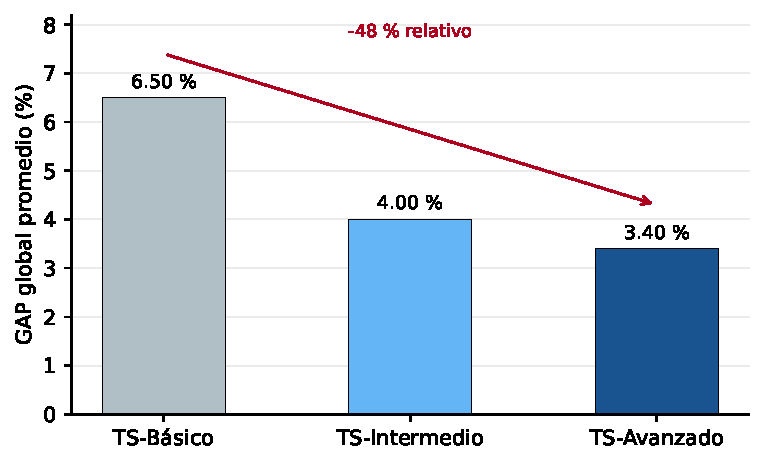
\includegraphics[width=0.72\linewidth]{gap_global.pdf}
  \caption{GAP global promedio por nivel de Búsqueda Tabú sobre los cinco
           problemas (360 experimentos, 5 semillas).}
  \label{fig:gap_global}
\end{figure}

El promedio global, sin embargo, oculta un efecto no uniforme. La
Figura~\ref{fig:gap_problema} desagrega por problema en escala logarítmica:
CVRP concentra casi toda la ganancia (de \SI{19.22}{\percent} a
\SI{6.38}{\percent}), mientras que en Flowshop los tres niveles quedan en
torno al \SI{1.7}{\percent} y la diferencia entre ellos es marginal.

\begin{figure}[H]
  \centering
  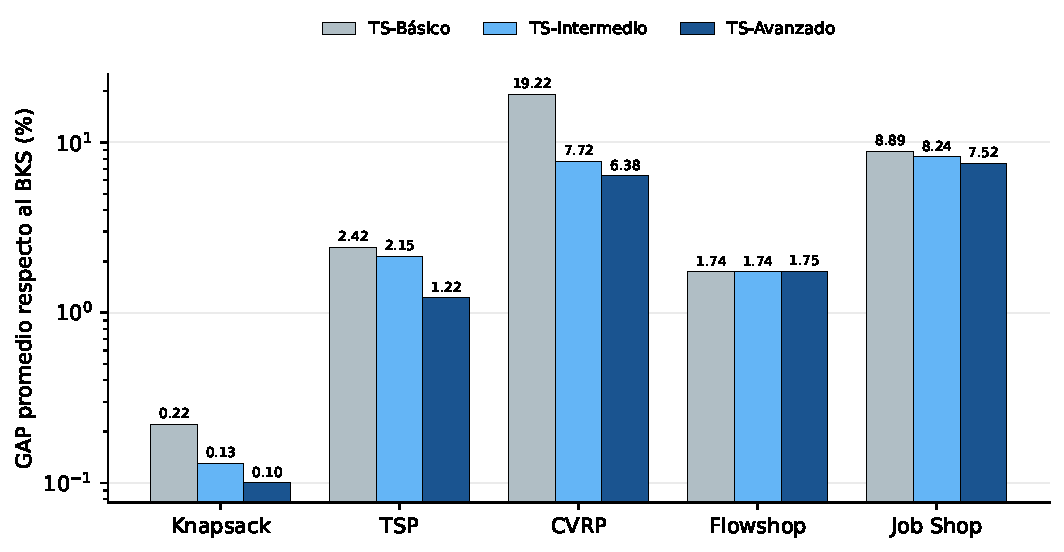
\includegraphics[width=\linewidth]{gap_por_problema.pdf}
  \caption{GAP promedio por problema y nivel (escala logarítmica). El efecto
           de los mecanismos de memoria depende fuertemente del problema.}
  \label{fig:gap_problema}
\end{figure}

Esa heterogeneidad es, en sí misma, un resultado: los mecanismos de memoria
de largo plazo rinden donde el espacio de búsqueda es amplio y accidentado
(CVRP, Job Shop), y aportan poco donde la vecindad deja escaso margen sobre la
solución constructiva (Flowshop con NEH e intercambio adyacente, Knapsack
con \emph{greedy} por ratio).

La mejora no es gratuita. La Figura~\ref{fig:calidad_tiempo} sitúa cada nivel
en el plano calidad--costo: TS-Avanzado requiere aproximadamente
$3.9\times$ el tiempo de TS-Básico para obtener cerca de la mitad del GAP.

\begin{figure}[H]
  \centering
  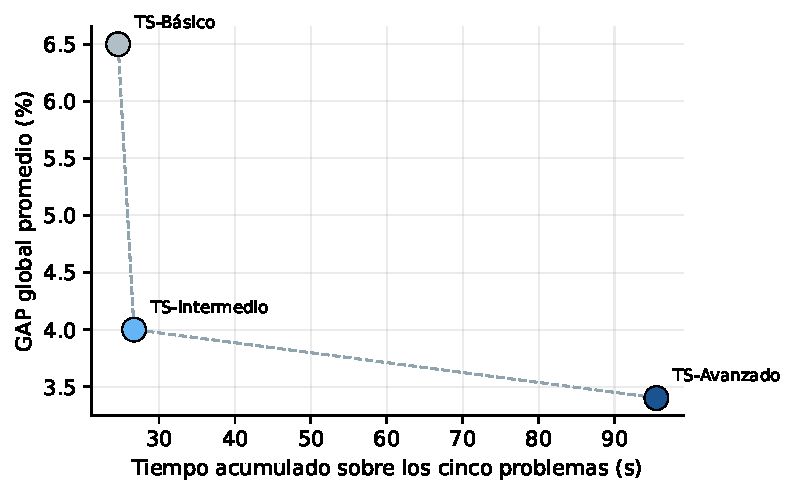
\includegraphics[width=0.72\linewidth]{calidad_vs_tiempo.pdf}
  \caption{Compromiso entre calidad de solución y costo computacional
           acumulado sobre los cinco problemas.}
  \label{fig:calidad_tiempo}
\end{figure}

Finalmente, la Figura~\ref{fig:dispersion} muestra la desviación estándar del
GAP entre las cinco semillas. La baja dispersión en la mayoría de las
instancias respalda que las diferencias observadas entre niveles no son ruido
muestral.

\begin{figure}[H]
  \centering
  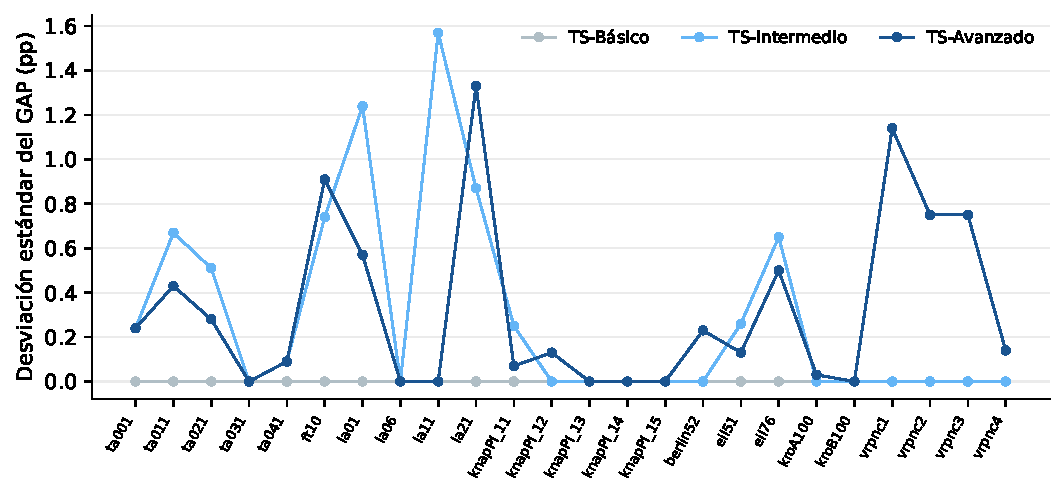
\includegraphics[width=\linewidth]{dispersion_semillas.pdf}
  \caption{Desviación estándar del GAP entre las cinco semillas
           $\{42, 123, 456, 789, 1337\}$, por instancia y nivel.}
  \label{fig:dispersion}
\end{figure}

\section{Contribuciones}

Mientras los objetivos de la Sección~\ref{sec:objetivos} declaran la intención,
esta sección enuncia lo efectivamente obtenido:

\begin{enumerate}
  \item \textbf{Una medición de la contribución de cada mecanismo.} La progresión de
    TS-Básico a TS-Avanzado reduce el GAP global de \SI{6.50}{\percent} a
    \SI{3.40}{\percent}, y el trabajo establece cuánto de esa reducción
    corresponde a cada componente: 2.50 puntos porcentuales a la lista tabú
    dinámica y 0.60 a los mecanismos de memoria de largo plazo.
  \item \textbf{La constatación de un efecto no uniforme.} La ganancia
    se concentra en los problemas de espacio de búsqueda amplio —CVRP reduce
    su GAP un \SI{67}{\percent} relativo— y resulta marginal donde la
    vecindad deja escaso margen sobre la solución constructiva. Esto acota
    cuándo conviene pagar el costo de los mecanismos avanzados.
  \item \textbf{Un criterio de decisión práctico.} TS-Avanzado exige
    aproximadamente $3.9\times$ el tiempo de TS-Básico para obtener cerca de
    la mitad del GAP, mientras TS-Intermedio captura el \SI{81}{\percent} de la mejora
    total a una fracción de ese costo.
  \item \textbf{Un repositorio público y reproducible} con las quince
    implementaciones, el orquestador de los 360 experimentos, modelos exactos
    de verificación y los resultados persistidos, extensible a nuevos
    problemas o algoritmos sin modificar la infraestructura existente.
\end{enumerate}

\section{Estructura del documento}
\label{sec:estructura}

El resto del documento se organiza en cinco capítulos:

\begin{itemize}
  \item El \textbf{Capítulo~\ref{cap:metodologia}} describe la metodología
    de trabajo: el diseño factorial, las decisiones que delimitan el
    estudio, las instancias de prueba, el protocolo experimental y los
    controles de validación.
  \item El \textbf{Capítulo~\ref{cap:paper}} incluye el artículo en formato
    IEEE, con el marco teórico de los cinco problemas, el pseudocódigo de
    los tres niveles de Búsqueda Tabú y los resultados desagregados por
    problema.
  \item El \textbf{Capítulo~\ref{cap:afiche}} presenta el afiche con que el
    trabajo se expuso en EXPOTIC UNAB 2026.
  \item El \textbf{Capítulo~\ref{cap:repositorio}} documenta el repositorio
    desde la ingeniería de software: requisitos, arquitectura, componentes,
    uso y extensión.
  \item El \textbf{Capítulo~\ref{cap:conclusion}} resume los hallazgos, las
    limitaciones y el trabajo futuro.
\end{itemize}

% =======================================================================
\chapter{Metodología de trabajo}
\label{cap:metodologia}
% =======================================================================

Este capítulo describe cómo se construyó el trabajo: las decisiones de diseño
que delimitaron el estudio, el protocolo experimental y los criterios de
validación. El detalle formal de los algoritmos y el análisis de resultados
se encuentran en el paper del Capítulo~\ref{cap:paper}.

\section{Enfoque general}

El trabajo sigue un diseño factorial completo de dos factores:

\begin{itemize}
  \item \textbf{Factor A --- Problema} (5 niveles): Knapsack 0/1, TSP, CVRP,
    Flowshop y Job Shop.
  \item \textbf{Factor B --- Configuración de TS} (3 niveles): Básico,
    Intermedio y Avanzado.
\end{itemize}

El cruce produce quince módulos independientes. Sobre cada módulo se ejecutan
las instancias correspondientes y cinco semillas, para un total de
\textbf{360 experimentos} (Figura~\ref{fig:diseno_factorial}). La estructura
factorial permite atribuir diferencias al mecanismo y no al problema: al
mantener fija la instancia y variar solo el nivel, la diferencia de GAP mide
la contribución del mecanismo añadido.

\begin{figure}[H]
  \centering
  \begin{tikzpicture}[x=1cm, y=0.82cm,
      celda/.style={draw, minimum width=2.45cm, minimum height=0.58cm,
                    fill=gray!10, font=\footnotesize, inner sep=1pt},
      fila/.style={font=\footnotesize, anchor=west},
      tot/.style={font=\footnotesize, anchor=west}]
    % Encabezados
    \node[font=\footnotesize\bfseries] at (5.8,1.55)
      {Factor B --- Configuración de TS};
    \foreach \x/\n in {3.2/TS-Básico, 5.8/TS-Intermedio, 8.4/TS-Avanzado}
      \node[font=\footnotesize\bfseries] at (\x,0.85) {\n};
    \node[font=\footnotesize\bfseries, anchor=west] at (-2.7,0.85)
      {Factor A --- Problema};
    \node[font=\footnotesize\bfseries, anchor=west] at (10.1,0.85) {Total};
    % Filas: problema, instancias, corridas por celda, total por fila
    \foreach \y/\prob/\inst/\cel/\fil in {
        0/Knapsack 0\slash 1/5/25/75,
        -1/TSP/5/25/75,
        -2/CVRP/4/20/60,
        -3/Flowshop/5/25/75,
        -4/Job Shop/5/25/75}{
      \node[fila] at (-2.7,\y) {\prob\ (\inst\ instancias)};
      \foreach \x in {3.2, 5.8, 8.4}
        \node[celda] at (\x,\y) {\cel\ corridas};
      \node[tot] at (10.1,\y) {\fil};
    }
    % Total general
    \draw (-2.7,-4.65) -- (11.0,-4.65);
    \node[fila] at (-2.7,-5.15)
      {24 instancias $\times$ 3 niveles $\times$ 5 semillas};
    \node[tot, font=\footnotesize\bfseries] at (10.1,-5.15) {360};
  \end{tikzpicture}
  \caption{Diseño factorial del estudio. Cada celda es un módulo de Búsqueda
           Tabú (problema $\times$ nivel); sus corridas resultan de ejecutar
           cada instancia del problema con las cinco semillas.}
  \label{fig:diseno_factorial}
\end{figure}

\section{Decisiones de diseño}

Cuatro decisiones delimitan el estudio: comparar tres niveles acumulativos en
lugar de barrer parámetros, trabajar con cinco problemas de estructura
distinta, restringir el tamaño de las instancias y emplear únicamente
benchmarks públicos con mejor valor conocido. Las subsecciones siguientes
justifican cada una.

\subsection{Por qué tres niveles y no un barrido de parámetros}

Un barrido exhaustivo de hiperparámetros habría producido mejores GAP
absolutos, pero habría confundido el objetivo. Aquí interesa el efecto de
\emph{agregar un mecanismo}, no especificarlo en detalle. Por eso los tres
niveles son acumulativos —cada uno contiene al anterior más un componente
adicional— y los parámetros se fijan una única vez por problema, sin
re-ajuste por instancia.

\subsection{Por qué esos cinco problemas}

Los cinco problemas se seleccionaron por su heterogeneidad estructural. Cada
uno representa una familia distinta de POC —selección, ruteo y
secuenciación— y obliga a una codificación y a una vecindad propias
(Tabla~\ref{tab:problemas}). Los cinco son, además, problemas clásicos con
benchmarks públicos y mejor valor conocido documentado, requisito de la
métrica empleada. Un mecanismo que funciona en los cinco persigue una
generalidad que no tendría si se hubieran elegido cinco variantes de ruteo.

\subsection{Por qué instancias de tamaño moderado}

Se privilegiaron instancias de 50 a 150 elementos, que se obtienen de
benchmarks estándar. Instancias mayores habrían elevado el tiempo por
experimento por encima de la capacidad del hardware disponible (ver
Sección~\ref{sec:entorno}) y, con 360 corridas, el costo total se habría
vuelto prohibitivo. La contrapartida —que los resultados no informan sobre
escalabilidad— se reconoce explícitamente como limitación.

\subsection{Por qué benchmarks públicos con BKS conocido}

Usar instancias generadas \emph{ad hoc} habría impedido contrastar contra un valor
de referencia externo. Todas las instancias provienen de repositorios
públicos con mejor valor conocido (BKS) documentado~\cite{reinelt1991tsplib,
taillard1993benchmarks,christofides1979vehicle}. Esto permite expresar
el rendimiento como GAP y comparar entre problemas de unidades distintas.

\section{Instancias de prueba}

Se emplean 24 instancias. La Tabla~\ref{tab:instancias_tesis} resume su
procedencia; el detalle de tamaños y valores BKS está en el paper.

\begin{table}[H]
\centering
\caption{Origen de las instancias de prueba}
\label{tab:instancias_tesis}
\small
\begin{tabular}{llll}
\toprule
\textbf{Problema} & \textbf{Instancias} & \textbf{N.º} & \textbf{Fuente} \\
\midrule
Knapsack 0/1 & \texttt{knapPI\_11}--\texttt{knapPI\_15} & 5
             & Pisinger~\cite{pisinger2005hard} \\
TSP  & \texttt{eil51}, \texttt{berlin52}, \texttt{eil76},
       \texttt{kroA100}, \texttt{kroB100} & 5
     & TSPLIB~\cite{reinelt1991tsplib} \\
CVRP & \texttt{vrpnc1}--\texttt{vrpnc4} & 4
     & Christofides~\cite{christofides1979vehicle} \\
Flowshop & \texttt{ta001}, \texttt{ta011}, \texttt{ta021},
           \texttt{ta031}, \texttt{ta041} & 5
         & Taillard~\cite{taillard1993benchmarks} \\
Job Shop & \texttt{ft10} & 1
         & Fisher \& Thompson~\cite{fisher1963probabilistic} \\
         & \texttt{la01}, \texttt{la06}, \texttt{la11}, \texttt{la21} & 4
         & Lawrence~\cite{lawrence1984resource} \\
\midrule
\multicolumn{2}{l}{\textbf{Total}} & \textbf{24} & \\
\bottomrule
\end{tabular}
\end{table}

\section{Protocolo experimental}

El protocolo fija cuatro elementos antes de ejecutar los experimentos: la
solución inicial de cada problema, los parámetros de cada nivel, las semillas
junto con el criterio de parada, y la métrica de comparación. Fijarlos de
antemano asegura que los tres niveles se comparen en igualdad de condiciones.

\subsection{Soluciones iniciales}

Ningún nivel arranca desde una solución aleatoria. Cada problema emplea una
heurística constructiva determinista; así, la comparación entre niveles no
se distorsiona por la calidad del punto de partida:

\begin{table}[H]
\centering
\caption{Heurística constructiva por problema}
\label{tab:constructivas}
\small
\begin{tabular}{lp{9.2cm}}
\toprule
\textbf{Problema} & \textbf{Heurística inicial} \\
\midrule
Knapsack 0/1 & \emph{Greedy} por ratio ganancia/peso decreciente \\
TSP          & Vecino más cercano desde el nodo 0~\cite{johnson1997traveling} \\
CVRP         & Ahorros de Clarke-Wright~\cite{clarke1964scheduling} \\
Flowshop     & NEH (Nawaz, Enscore \& Ham)~\cite{nawaz1983heuristic} \\
Job Shop     & Decodificador Giffler-Thompson~\cite{giffler1960algorithms} con
               prioridad por tiempo total de procesamiento decreciente \\
\bottomrule
\end{tabular}
\end{table}

Esta decisión tiene una consecuencia visible en los resultados: en Flowshop,
donde NEH entrega una solución inicial de buena calidad, los tres niveles
de TS con vecindad de intercambio adyacente la mejoran poco.

\subsection{Parámetros por nivel}

Los parámetros se fijan por problema y nivel antes de ejecutar los
experimentos. La Tabla~\ref{tab:parametros_tesis} los resume; $|\mathcal{T}|$
es el tamaño de la lista tabú, $T_{\max}$ el número de iteraciones y $L$ el
umbral de estancamiento que dispara el reinicio.

\begin{table}[H]
\centering
\caption{Parámetros por problema y nivel}
\label{tab:parametros_tesis}
\small
\begin{tabular}{llccl}
\toprule
\textbf{Problema} & \textbf{Nivel} & $|\mathcal{T}|$ & $T_{\max}$ &
  \textbf{Reinicio} \\
\midrule
\multirow{3}{*}{Knapsack}
  & Básico  & 10 (fijo) & 500    & --- \\
  & Interm. & [5, 15]   & 1\,000 & $L=200$ \\
  & Avanz.  & [5, 15]   & 2\,000 & $L=200$, frecuencia \\
\midrule
\multirow{3}{*}{TSP}
  & Básico  & 10 (fijo) & 1\,000 & --- \\
  & Interm. & [5, 20]   & 2\,000 & $L=200$ \\
  & Avanz.  & [7, 25]   & 3\,000 & $L=300$, 4-opt \\
\midrule
\multirow{3}{*}{CVRP}
  & Básico  & 10 (fijo) & 1\,500 & --- \\
  & Interm. & [7, 20]   & 3\,000 & $L=300$ \\
  & Avanz.  & [7, 25]   & 5\,000 & $L=400$, frecuencia \\
\midrule
\multirow{3}{*}{Flowshop}
  & Básico  & 10 (fijo) & 2\,000 & --- \\
  & Interm. & [5, 20]   & 4\,000 & $L=500$ \\
  & Avanz.  & [5, 20]   & 5\,000 & $L=500$, frecuencia \\
\midrule
\multirow{3}{*}{Job Shop}
  & Básico  & 10 (fijo) & 2\,500 & --- \\
  & Interm. & [5, 15]   & 1\,000 & $L=200$ \\
  & Avanz.  & [5, 15]   & 1\,500 & $L=250$, frecuencia \\
\bottomrule
\end{tabular}
\end{table}

Nótese que en Job Shop el nivel Básico usa más iteraciones que los
posteriores. Es una decisión deliberada: el costo por iteración crece con la
lista dinámica, y mantener $T_{\max}$ constante habría hecho que los niveles
superiores consumieran un tiempo desproporcionado. El criterio fue igualar
aproximadamente el tiempo de cómputo, no el número de iteraciones.

\subsection{Semillas y criterio de parada}

Cada configuración se ejecuta con cinco semillas independientes,
$s \in \{42, 123, 456, 789, 1337\}$, y se reportan media y desviación
estándar. Aunque una corrida de TS es determinista una vez fijada la semilla,
esta gobierna los componentes estocásticos del algoritmo —desempates,
perturbaciones de reinicio y diversificación—. Cada semilla constituye así una corrida independiente.

Se eligen cinco semillas, y no un número mayor, como equilibrio entre el
costo computacional (360 experimentos) y la estimación de la variabilidad.
La baja desviación estándar observada (Figura~\ref{fig:dispersion}) respalda
esa elección.

El criterio de parada es el número máximo de iteraciones $T_{\max}$, sin
condición de convergencia adicional. Esto simplifica la comparación pero
implica que los tiempos no son directamente comparables entre problemas.

\subsection{Métrica de comparación}

Se emplea el GAP porcentual respecto al BKS definido en la
Ecuación~\ref{eq:gap_motivo}. Un GAP de \SI{0}{\percent} indica coincidencia exacta con el BKS. Un GAP negativo indicaría la \emph{superación} del BKS; no se observa en ninguno de los 360 experimentos. Las instancias de Flowshop se regeneran
desde las semillas publicadas por Taillard~\cite{taillard1993benchmarks}
(\texttt{instances/flowshop/generar\_taillard.py}) y sus BKS son
\emph{makespan} óptimos.

\section{Flujo de ejecución}

El experimento completo se ejecuta con un solo comando. El orquestador
recorre el producto cartesiano de problemas, instancias, algoritmos y
semillas, y persiste cada corrida en disco antes de agregar los resultados.
La Figura~\ref{fig:flujo_ejecucion} muestra ese flujo y el
Código~\ref{lst:orquestador}, su implementación.

\begin{figure}[H]
  \centering
  \begin{tikzpicture}[
      node distance=0.42cm,
      paso/.style={draw, rounded corners=2pt, align=center,
                   font=\footnotesize, text width=8.6cm,
                   minimum height=0.8cm, fill=gray!8},
      dec/.style={draw, diamond, aspect=3.4, align=center,
                  font=\footnotesize, inner sep=1pt, fill=gray!15},
      fl/.style={->, >=stealth, thick}]
    \node[paso] (cli)
      {\texttt{main.py -{}-all -{}-multi-seed}\\
       toma la siguiente combinación\\
       (semilla, problema, instancia, algoritmo)};
    \node[paso, below=of cli] (load)
      {\texttt{loader.py}: lee la instancia desde \texttt{instances/}\\
       y entrega la matriz de datos y el BKS};
    \node[paso, below=of load] (solve)
      {\texttt{runner.py}: importa el módulo de TS\\
       e invoca \texttt{solve(instance\_data, seed)}};
    \node[paso, below=of solve] (met)
      {\texttt{metrics.py}: calcula el GAP respecto al BKS};
    \node[paso, below=of met] (out)
      {Persiste la corrida en \texttt{output/}:\\
       \texttt{resultado.json} y \texttt{solucion.txt}};
    \node[dec, below=of out] (mas) {¿Quedan combinaciones?};
    \node[paso, below=of mas] (rep)
      {\texttt{reporter.py}: agrega las 360 corridas en \texttt{results/}\\
       (media y desviación estándar por instancia)};
    \node[paso, below=of rep] (fig)
      {\texttt{notebooks/} y \texttt{generar\_figuras.py}: tablas y figuras};
    \draw[fl] (cli) -- (load);
    \draw[fl] (load) -- (solve);
    \draw[fl] (solve) -- (met);
    \draw[fl] (met) -- (out);
    \draw[fl] (out) -- (mas);
    \draw[fl] (mas) -- node[right, font=\scriptsize]{no} (rep);
    \draw[fl] (rep) -- (fig);
    \draw[fl] (mas.east) -- ++(2.3,0)
      node[midway, above, font=\scriptsize]{sí} |- (cli.east);
  \end{tikzpicture}
  \caption{Flujo de ejecución del experimento completo. El ciclo superior se
           repite para las 360 combinaciones; la agregación y las figuras se
           generan una sola vez al final.}
  \label{fig:flujo_ejecucion}
\end{figure}

\lstinputlisting[caption={Orquestador de experimentos y opciones de línea de
comandos},label={lst:orquestador}]{codigos/05_orquestador.py}

El flujo de datos es lineal y sin estado compartido entre corridas:

\begin{enumerate}
  \item \texttt{loader.py} lee la instancia desde \texttt{instances/} y
    devuelve un diccionario con la matriz de datos y el BKS.
  \item \texttt{runner.py} invoca el \texttt{solve()} del módulo
    correspondiente con la semilla indicada.
  \item El resultado se persiste en
    \texttt{output/\{problema\}/\{instancia\}\_\{algoritmo\}\_\{fecha\}/}
    como \texttt{resultado.json} (valor, GAP, iteraciones, tiempo e historial
    de convergencia) y \texttt{solucion.txt}.
  \item \texttt{metrics.py} calcula el GAP y \texttt{reporter.py} agrega
    todas las corridas en \texttt{results/tabla\_consolidada.csv} con media y
    desviación estándar por instancia.
  \item Los cuadernos de \texttt{notebooks/} y el script
    \texttt{TESIS/generar\_figuras.py} producen las figuras a partir de esos
    CSV.
\end{enumerate}

Que cada corrida escriba su propio directorio con marca de tiempo permite
re-ejecutar experimentos sin sobrescribir resultados previos y auditar la
trazabilidad completa.

\section{Reproducibilidad}

La reproducción íntegra de los resultados requiere tres comandos:

\begin{verbatim}
pip install -r requirements.txt
python src/main.py --all --multi-seed
python src/main.py --report
\end{verbatim}

Los CSV consolidados de \texttt{results/} están versionados, de modo que el
análisis puede reproducirse sin volver a ejecutar los experimentos.
Los modelos exactos de \texttt{models/python\_exact/} permiten, además,
verificar de forma independiente el BKS de las instancias más pequeñas de
Knapsack, TSP y Flowshop.

\section{Entorno de ejecución}
\label{sec:entorno}

Los experimentos se ejecutaron en un equipo ASUS TUF Dash F15 con procesador
Intel Core i7 de undécima generación, \SI{8}{\giga\byte} de memoria RAM
DDR4-3200 y tarjeta gráfica NVIDIA GeForce RTX~3050. Los algoritmos son de
un solo hilo y no utilizan la GPU.

Estas capacidades limitaron el número de iteraciones en las instancias
mayores de CVRP y Job Shop, y son la razón por la que el criterio de parada
es de iteraciones fijas y no de tiempo de CPU fijo. Una comparación
metodológicamente más estricta usaría lo segundo; se deja indicado como
trabajo futuro.

\section{Validación}

La validez de las conclusiones descansa en cuatro controles:

\begin{itemize}
  \item \textbf{Semillas múltiples.} Cinco corridas independientes por
    configuración, con desviación estándar reportada por instancia.
  \item \textbf{Referencia externa.} Todas las instancias tienen BKS
    publicado, ajeno a este trabajo.
  \item \textbf{Verificación exacta parcial.} Los solvers de
    \texttt{models/python\_exact/} confirman el óptimo en las instancias
    pequeñas de Knapsack (programación dinámica~\cite{martello1990knapsack}),
    TSP (Held-Karp~\cite{held1962dynamic}) y Flowshop.
  \item \textbf{Persistencia y trazabilidad.} Cada corrida escribe en
    \texttt{output/} su propio directorio con marca de tiempo, y los CSV
    consolidados de \texttt{results/} —versionados en su totalidad— respaldan
    todas las cifras de este documento. El repositorio distribuye además un
    subconjunto representativo de las corridas crudas; el conjunto completo se
    regenera con un solo comando.
\end{itemize}

% =======================================================================
\chapter{Paper}
\label{cap:paper}
% =======================================================================

Este capítulo reproduce íntegramente el artículo \emph{Triple Enfoque
Resolutivo: Un Repositorio de Cinco Problemas de Optimización Combinatoria
con Soluciones Exactas y Metaheurísticas}, en formato IEEE de conferencia.

El artículo se incluye tal como fue compilado, sin re-maquetación, para
preservar el formato de publicación. Contiene el marco teórico completo de
los cinco problemas y los tres niveles de Búsqueda Tabú, el diseño
experimental formal, los resultados desagregados por problema con sus tablas
y curvas de convergencia, y las conclusiones del estudio.

\begin{table}[H]
\centering
\caption{Contenido del artículo incluido}
\label{tab:contenido_paper}
\small
\begin{tabular}{ll}
\toprule
\textbf{Sección} & \textbf{Contenido} \\
\midrule
Resumen        & Síntesis y resultados principales \\
Introducción   & Contexto, brecha metodológica y contribuciones \\
Marco teórico  & Los cinco problemas y los tres niveles de TS, con
                 pseudocódigo \\
Diseño experimental & Estructura del repositorio, instancias, métricas \\
Resultados     & Análisis por problema y análisis global \\
Conclusiones   & Hallazgos de implementación y trabajo futuro \\
\bottomrule
\end{tabular}
\end{table}

\vfill
\noindent\textbf{Fuente:} \texttt{paper/main.pdf} del repositorio.
Para recompilarlo:
\texttt{cd paper \&\& pdflatex main.tex \&\& bibtex main \&\& pdflatex main.tex}.

\cleardoublepage

% --- Artículo completo, 9 páginas ---
\includepdf[pages=-,
            frame=false,
            scale=0.92,
            pagecommand={\thispagestyle{plain}}]%
           {../paper/main.pdf}

% =======================================================================
\chapter{Afiche EXPOTIC}
\label{cap:afiche}
% =======================================================================

El trabajo fue presentado en formato de póster académico en \textbf{EXPOTIC
UNAB 2026}, la muestra de proyectos de la Escuela de Ingeniería Informática
de la Universidad Andrés Bello.

El afiche condensa en una página el planteamiento del problema, la
arquitectura del repositorio, los tres niveles de Búsqueda Tabú y los
resultados principales de los 360 experimentos. Su función es distinta a la
del artículo: mientras el paper argumenta, el póster comunica: prioriza la
lectura rápida y el impacto visual sobre el detalle metodológico.

\begin{table}[H]
\centering
\caption{Ficha del afiche}
\label{tab:ficha_afiche}
\small
\begin{tabular}{ll}
\toprule
\textbf{Título} & Póster académico EXPOTIC UNAB 2026 \\
\textbf{Autor} & Benjamín Peña Díaz \\
\textbf{Instancia} & EXPOTIC, Universidad Andrés Bello, 2026 \\
\textbf{Formato} & A4 vertical, una página \\
\textbf{Archivo} & \texttt{EXPOTIC/afiche-triple-enfoque-resolutivo.pdf} \\
\bottomrule
\end{tabular}
\end{table}

La carpeta \texttt{EXPOTIC/} del repositorio contiene además el material
complementario de la presentación: la versión fuente del afiche
(\texttt{afiche/afiche.html}), el artículo en formato de la plantilla del
evento (\texttt{articulo/}) y la presentación de apoyo
(\texttt{presentation\_EN.pptx} y su versión en PDF).

El afiche se reproduce tal como se presentó en el evento. Sus cifras de
Flowshop y de GAP global corresponden a una versión anterior de los
experimentos; los valores vigentes, obtenidos con las instancias de Taillard
regeneradas desde sus semillas publicadas, son los que se reportan en el
resto de este documento.

\cleardoublepage

% --- Afiche, 1 página A4 ---
% Se usa \thispagestyle{empty}: el afiche tiene fondo oscuro a sangre y el
% número de página quedaría ilegible sobre él.
\includepdf[pages=-,
            fitpaper=false,
            scale=0.94,
            pagecommand={\thispagestyle{empty}}]%
           {../EXPOTIC/afiche-triple-enfoque-resolutivo.pdf}

% =======================================================================
\chapter{El repositorio}
\label{cap:repositorio}
% =======================================================================

El repositorio \texttt{Triple-Resolutive-Approach-repo} es el producto
central de este trabajo. No acompaña al paper: lo sostiene. Todas las cifras
del Capítulo~\ref{cap:paper} se derivan de artefactos que están versionados
en él, y cualquiera de ellas puede rastrearse hasta la corrida individual que
la produjo.

Este capítulo lo documenta desde la ingeniería de software: los principios
que guiaron su diseño, los requisitos que satisface, su arquitectura
—descrita con diagramas UML—, sus componentes, su uso y cómo extenderlo.

\section{Principios de diseño}

Tres decisiones estructurales explican la forma del repositorio:

\begin{description}
  \item[Interfaz uniforme.] Los quince módulos de Búsqueda Tabú exponen la
    misma función \texttt{solve()} y devuelven el mismo diccionario
    (Código~\ref{lst:interfaz}). El orquestador no contiene ninguna
    ramificación por problema.
  \item[Separación entre algoritmo e infraestructura.] Los módulos de
    \texttt{tabu\_search/} no saben nada de archivos, formatos ni métricas.
    Reciben un diccionario de datos y devuelven un diccionario de resultados.
    Toda la entrada/salida vive en \texttt{src/}.
  \item[Persistencia inmutable.] Cada corrida escribe su propio directorio con
    marca de tiempo. Nada se sobrescribe, de modo que re-ejecutar experimentos
    nunca destruye evidencia previa.
\end{description}

\section{Requisitos}
\label{sec:requisitos}

Los objetivos de la Sección~\ref{sec:objetivos} se traducen en los requisitos
de la Tabla~\ref{tab:requisitos}. Los funcionales describen qué debe hacer el
repositorio; los de calidad, cómo debe hacerlo~\cite{bass2012software}. La
última columna indica el componente que satisface cada uno.

\begin{table}[H]
\centering
\caption{Requisitos del repositorio y componente que los satisface}
\label{tab:requisitos}
\small
\begin{tabular}{lp{8.3cm}p{3.7cm}}
\toprule
\textbf{ID} & \textbf{Requisito} & \textbf{Componente} \\
\midrule
\multicolumn{3}{l}{\emph{Requisitos funcionales}} \\
RF1 & Ejecutar una combinación cualquiera de problema, instancia, nivel de
      TS y semilla desde la línea de comandos.
    & \texttt{main.py}, \texttt{runner.py} \\
RF2 & Ejecutar el diseño factorial completo (360 experimentos) con un solo
      comando.
    & \texttt{main.py} \\
RF3 & Persistir cada corrida con su valor, GAP, tiempo, historial de
      convergencia y solución.
    & \texttt{runner.py}, \texttt{output/} \\
RF4 & Consolidar las corridas en tablas con media y desviación estándar por
      instancia.
    & \texttt{reporter.py}, \texttt{results/} \\
RF5 & Verificar de forma independiente el óptimo de las instancias pequeñas.
    & \texttt{models/} \\
\midrule
\multicolumn{3}{l}{\emph{Requisitos de calidad}} \\
RC1 & Reproducibilidad: semillas fijas y dependencias con versión declarada.
    & \texttt{main.py}, \texttt{requirements.txt} \\
RC2 & Extensibilidad: agregar un problema o un nivel de TS sin modificar el
      orquestador.
    & interfaz \texttt{solve()} \\
RC3 & Trazabilidad: toda cifra publicada se rastrea hasta las corridas que
      la producen.
    & \texttt{output/}, \texttt{results/} \\
RC4 & Bajo acoplamiento: \texttt{solve()} recibe y devuelve diccionarios,
      sin leer ni escribir archivos.
    & \texttt{tabu\_search/} \\
\bottomrule
\end{tabular}
\end{table}

\section{Arquitectura de software}
\label{sec:arquitectura}

La arquitectura separa tres responsabilidades: la orquestación de los
experimentos, los algoritmos de Búsqueda Tabú y los servicios de
infraestructura (carga de instancias, métricas y reportes). Se documenta con
dos vistas UML~\cite{fowler2003uml}: una estructural y una de comportamiento.

\subsection{Vista estructural: diagrama de clases}

El repositorio se organiza en módulos de funciones y no en clases. Por eso,
en la Figura~\ref{fig:uml_clases_tesis} cada módulo se modela como una clase
con el estereotipo «módulo», cuyas operaciones son sus funciones públicas
(\texttt{+}) y privadas (\texttt{-}). La interfaz \texttt{SolverTS} no existe
como archivo: representa el contrato que cumplen los quince módulos de
\texttt{tabu\_search/}.

\begin{figure}[H]
  \centering
  \begin{tikzpicture}[
      clase/.style={draw, rectangle split, rectangle split parts=2,
                    align=left, font=\footnotesize\ttfamily, fill=gray!8,
                    inner sep=3pt, text width=6.7cm, anchor=north},
      dep/.style={->, >=stealth, dashed},
      real/.style={-{Triangle[open, length=6pt, width=7pt]}, dashed},
      rot/.style={font=\scriptsize\itshape, text=gray!90!black}]
    % Columna izquierda: orquestación y algoritmos
    \node[clase] (main) at (0,0)
      {\centering «módulo»\\\textbf{src/main.py}
       \nodepart{two}+ DEFAULT\_SEEDS: list[int]\\
       + main(): None\\
       + run\_all(seeds, verbose): None\\
       - \_list\_instances(problema): list[str]};
    \node[clase] (run) at (0,-3.3)
      {\centering «módulo»\\\textbf{src/runner.py}
       \nodepart{two}+ PROBLEMS, ALGORITHMS, EXTENSIONS\\
       + run\_experiment(problema, instancia,\\
       \ \ \ algoritmo, seed): dict\\
       - \_find\_instance\_file(...)\\
       - \_load\_solver(problema, algoritmo)\\
       - \_make\_output\_dir(...)};
    \node[clase] (ifz) at (0,-7.5)
      {\centering «interface»\\\textbf{SolverTS}
       \nodepart{two}+ solve(instance\_data, ..., seed): dict};
    \node[clase] (impl) at (0,-9.75)
      {\centering «módulo»\\\textbf{tabu\_search/\{problema\}/}
       \nodepart{two}ts\_basico.py\\ts\_intermedio.py\\ts\_avanzado.py};
    % Columna derecha: servicios de infraestructura
    \node[clase] (rep) at (7.7,0)
      {\centering «módulo»\\\textbf{src/reporter.py}
       \nodepart{two}+ generate\_report(verbose): None\\
       - \_load\_results(): list[dict]\\
       - \_aggregate\_results(records): dict\\
       - \_write\_consolidated(...)};
    \node[clase] (load) at (7.7,-3.3)
      {\centering «módulo»\\\textbf{src/loader.py}
       \nodepart{two}+ load\_instance(filepath): dict\\
       + load\_knapsack(filepath): dict\\
       + load\_tsp(filepath): dict\\
       + load\_vrp(filepath): dict\\
       + load\_flowshop(filepath): dict\\
       + load\_jobshop(filepath): dict};
    \node[clase] (met) at (7.7,-7.5)
      {\centering «módulo»\\\textbf{src/metrics.py}
       \nodepart{two}+ MINIMIZATION: dict[str, bool]\\
       + gap(value, bks, minimization): float\\
       + summarize(result, instance\_data,\\
       \ \ \ problema): dict};
    % Dependencias y realización
    \draw[dep] (main) -- (rep);
    \draw[dep] (main) -- (run);
    \draw[dep] (run) -- (load);
    \draw[dep] (run) -- node[right, rot]{importación dinámica} (ifz);
    \draw[dep] (run.south east) -- (met.north west);
    \draw[real] (impl) -- node[right, rot]{5 problemas $\times$ 3 niveles} (ifz);
  \end{tikzpicture}
  \caption{Diagrama de clases UML del repositorio. Las flechas punteadas
           indican dependencia; la flecha con triángulo hueco, la realización
           de la interfaz \texttt{solve()} por los quince módulos de TS.}
  \label{fig:uml_clases_tesis}
\end{figure}

El diagrama muestra tres propiedades de la arquitectura:

\begin{itemize}
  \item \texttt{runner.py} concentra las dependencias: usa
    \texttt{loader.py}, \texttt{metrics.py} y la interfaz \texttt{SolverTS},
    pero no conoce ningún módulo de TS en particular.
  \item \texttt{reporter.py} no depende de \texttt{runner.py}. Ambos se
    comunican a través de los archivos de \texttt{output/}; por eso el
    reporte puede regenerarse sin volver a ejecutar los experimentos.
  \item \texttt{loader.py} oculta los cinco formatos de instancia tras una
    única función, \texttt{load\_instance()}, que elige el \emph{parser}
    según la extensión del archivo.
\end{itemize}

\subsection{Patrones de diseño}

Dos decisiones de diseño explican el requisito de extensibilidad (RC2):

\begin{itemize}
  \item \textbf{Estrategia.} Los quince módulos de TS son estrategias
    intercambiables tras una misma firma, \texttt{solve()}, en el sentido del
    patrón \emph{Strategy}~\cite{gamma1994design}. El código cliente
    —\texttt{runner.py}— trata por igual a los tres niveles y a los cinco
    problemas.
  \item \textbf{Carga dinámica.} \texttt{runner.py} construye el nombre del
    módulo a partir del problema y del algoritmo —por ejemplo,
    \texttt{tabu\_search.\allowbreak tsp.\allowbreak ts\_basico}— y lo
    importa en tiempo de ejecución con \texttt{importlib}. Agregar una estrategia nueva
    exige crear un archivo y registrar su nombre, sin tocar el orquestador.
\end{itemize}

\subsection{Vista de comportamiento: diagrama de secuencia}

La Figura~\ref{fig:uml_secuencia} muestra la interacción entre los módulos
durante un experimento individual, es decir, una llamada a
\texttt{run\_experiment()}. El experimento completo repite esta secuencia
para cada una de las 360 combinaciones (Figura~\ref{fig:flujo_ejecucion}).

\begin{figure}[H]
  \centering
  \begin{tikzpicture}[
      obj/.style={draw, fill=gray!8, font=\footnotesize\ttfamily,
                  minimum height=0.62cm, minimum width=2.05cm,
                  text height=1.6ex, text depth=0.4ex},
      vida/.style={dashed, gray!70},
      msg/.style={->, >=stealth, thick},
      ret/.style={->, >=stealth, dashed},
      etq/.style={font=\scriptsize\ttfamily, fill=white, inner sep=1.2pt}]
    % Participantes
    \node[obj] (m)  at (0,0)    {main.py};
    \node[obj] (r)  at (3.1,0)  {runner.py};
    \node[obj] (l)  at (6.2,0)  {loader.py};
    \node[obj] (t)  at (9.3,0)  {módulo TS};
    \node[obj] (me) at (12.4,0) {metrics.py};
    % Líneas de vida
    \foreach \o in {m,r,l,t,me}
      \draw[vida] (\o.south) -- ++(0,-8.75);
    % Activación de runner.py
    \draw[fill=gray!25] (3.0,-1.0) rectangle (3.2,-8.6);
    % 1. main -> runner
    \draw[msg] (0,-1.0) -- (3.0,-1.0);
    \node[etq, anchor=south west] at (0.1,-0.97) {run\_experiment(...)};
    % 2. runner -> loader
    \draw[msg] (3.2,-1.95) -- (6.2,-1.95);
    \node[etq, anchor=south west] at (3.3,-1.92) {load\_instance(ruta)};
    \draw[ret] (6.2,-2.6) -- (3.2,-2.6);
    \node[etq, anchor=south west] at (3.3,-2.57) {instance\_data (datos y BKS)};
    % 3. runner -> runner (importación dinámica)
    \draw[msg] (3.2,-3.35) -- ++(0.7,0) -- ++(0,-0.4) -- (3.2,-3.75);
    \node[etq, anchor=west] at (4.0,-3.55)
      {\_load\_solver(problema, algoritmo): importación dinámica};
    % 4. runner -> módulo TS
    \draw[msg] (3.2,-4.7) -- (9.3,-4.7);
    \node[etq, anchor=south west] at (3.3,-4.67) {solve(instance\_data, seed=seed)};
    \draw[ret] (9.3,-5.35) -- (3.2,-5.35);
    \node[etq, anchor=south west] at (3.3,-5.32)
      {\{value, solution, iterations, time\_s, history\}};
    % 5. runner -> metrics
    \draw[msg] (3.2,-6.25) -- (12.4,-6.25);
    \node[etq, anchor=south west] at (3.3,-6.22)
      {summarize(result, instance\_data, problema)};
    \draw[ret] (12.4,-6.9) -- (3.2,-6.9);
    \node[etq, anchor=south west] at (3.3,-6.87)
      {\{value, bks, gap\_pct, iterations, time\_s\}};
    % 6. runner -> runner (persistencia)
    \draw[msg] (3.2,-7.5) -- ++(0.7,0) -- ++(0,-0.4) -- (3.2,-7.9);
    \node[etq, anchor=west] at (4.0,-7.7)
      {escribe resultado.json y solucion.txt en output/};
    % 7. retorno a main
    \draw[ret] (3.0,-8.6) -- (0,-8.6);
    \node[etq, anchor=south west] at (0.1,-8.57) {dict};
  \end{tikzpicture}
  \caption{Diagrama de secuencia UML de un experimento individual. Las
           flechas continuas son llamadas; las punteadas, valores de retorno.}
  \label{fig:uml_secuencia}
\end{figure}

\section{Estructura de directorios}

\begin{figure}[H]
\footnotesize
\begin{verbatim}
Triple-Resolutive-Approach-repo/
|- instances/          Instancias benchmark (24 archivos)
|  |- knapsack/  .kp     tsp/  .tsp      vrp/  .vrp
|  `- flowshop/  .fsp    jobshop/ .jss
|- models/
|  |- ampl/            5 modelos AMPL de referencia exacta (.mod)
|  `- python_exact/    Solvers exactos: Knapsack DP, TSP Held-Karp, Flowshop
|- tabu_search/        15 modulos: 5 problemas x 3 niveles
|  |- knapsack/  ts_basico.py  ts_intermedio.py  ts_avanzado.py
|  `- tsp/  vrp/  flowshop/  jobshop/   (misma estructura)
|- src/
|  |- loader.py        Parsers de instancias y BKS
|  |- runner.py        Ejecutor de un experimento individual
|  |- metrics.py       Calculo de GAP y metricas
|  |- reporter.py      Consolidacion en CSV y tablas LaTeX
|  |- main.py          CLI principal
|  |- tables/          Tablas LaTeX por instancia (generadas)
|  `- utils/           Utilidades de exportacion de tablas
|- output/             Resultados crudos: un directorio por corrida
|- results/            CSVs consolidados por problema y global
|- notebooks/          5 cuadernos Jupyter de analisis
|- paper/              Paper IEEE en LaTeX (main.tex + secciones/ + figuras/)
|- EXPOTIC/            Afiche, articulo y presentacion del evento
|- TESIS/              Este documento
`- requirements.txt
\end{verbatim}
\caption{Estructura del repositorio.}
\label{fig:estructura_repo}
\end{figure}

\section{Componentes}

\subsection{\texttt{instances/} --- las entradas}

Contiene las 24 instancias benchmark en su formato original, con una
extensión por problema (\texttt{.kp}, \texttt{.tsp}, \texttt{.vrp},
\texttt{.fsp}, \texttt{.jss}). Los archivos no fueron modificados respecto a
la fuente, de modo que pueden contrastarse contra los repositorios públicos
originales.

\subsection{\texttt{tabu\_search/} --- los algoritmos}

El corazón del repositorio: quince módulos organizados en cinco carpetas, una
por problema, cada una con \texttt{ts\_basico.py}, \texttt{ts\_intermedio.py}
y \texttt{ts\_avanzado.py}. Cada módulo es autocontenido —implementa su propia
vecindad, su lista tabú y su heurística constructiva— y no importa nada de los
demás.

La progresión entre niveles se aprecia en el tamaño del código y en la
naturaleza de la memoria empleada: TS-Básico mantiene una \texttt{deque} de
tamaño fijo (Código~\ref{lst:basico}), mientras TS-Avanzado añade una matriz
de frecuencia, un parámetro de penalización adaptativo y un mecanismo de
perturbación estructural (Código~\ref{lst:avanzado}).

Cada módulo es además ejecutable directamente, lo que permite probar un
algoritmo sobre todas las instancias de su problema sin pasar por el
orquestador:

\begin{verbatim}
python tabu_search/tsp/ts_avanzado.py
\end{verbatim}

\subsection{\texttt{src/} --- la infraestructura}

Cinco módulos con responsabilidades disjuntas:

\begin{table}[H]
\centering
\caption{Módulos de infraestructura}
\label{tab:modulos_src}
\small
\begin{tabular}{llp{7cm}}
\toprule
\textbf{Módulo} & \textbf{Líneas} & \textbf{Responsabilidad} \\
\midrule
\texttt{loader.py}   & 392 & Parsers de los cinco formatos de instancia.
  Devuelve un diccionario con la matriz de datos y el BKS documentado. \\
\texttt{runner.py}   & 194 & Ejecuta un experimento individual: carga la
  instancia, importa dinámicamente el módulo de TS, invoca \texttt{solve()}
  y persiste el resultado. \\
\texttt{metrics.py}  &  68 & Cálculo del GAP respecto al BKS, con manejo del
  signo según sea problema de minimización o maximización
  (Código~\ref{lst:gap}). \\
\texttt{reporter.py} & 324 & Recorre \texttt{output/}, agrega por instancia
  y nivel, y genera los CSV de \texttt{results/} y las tablas LaTeX de
  \texttt{src/tables/}. \\
\texttt{main.py}     & 193 & Interfaz de línea de comandos y orquestación del
  producto cartesiano completo (Código~\ref{lst:orquestador}). \\
\bottomrule
\end{tabular}
\end{table}

La importación dinámica en \texttt{runner.py} es el detalle que hace
extensible el sistema: el nombre del módulo se construye a partir de los
argumentos \texttt{problema} y \texttt{algoritmo}, de modo que agregar un
módulo nuevo lo hace inmediatamente ejecutable sin tocar el orquestador.

\subsection{\texttt{models/} --- verificación independiente}

Dos vías de verificación del BKS:

\begin{itemize}
  \item \texttt{models/ampl/} --- cinco modelos exactos en AMPL
    (\texttt{knapsack.mod}, \texttt{tsp\_mtz.mod}, \texttt{cvrp.mod},
    \texttt{flowshop.mod}, \texttt{jobshop\_manne.mod}). Requieren licencia
    de AMPL.
  \item \texttt{models/python\_exact/} --- tres solvers exactos ejecutables
    sin dependencias comerciales: programación dinámica para Knapsack,
    Held-Karp para TSP y enumeración acotada para Flowshop. Permiten
    confirmar el óptimo en las instancias pequeñas.
\end{itemize}

\subsection{\texttt{output/} y \texttt{results/} --- la evidencia}

\texttt{output/} almacena los resultados crudos: un directorio por corrida,
nombrado \texttt{\{instancia\}\_\{algoritmo\}\_\{fecha\}/}, con dos archivos:

\begin{itemize}
  \item \texttt{resultado.json} --- valor obtenido, BKS, GAP, iteraciones,
    tiempo e historial completo de convergencia.
  \item \texttt{solucion.txt} --- la mejor solución encontrada en formato
    legible.
\end{itemize}

El historial de convergencia es lo que permite reconstruir las curvas del
paper sin re-ejecutar nada. \texttt{results/} contiene la vista agregada: un
CSV por problema más \texttt{tabla\_consolidada.csv}, con media y desviación
estándar del GAP y del tiempo sobre las cinco semillas.

Conviene precisar el alcance del material distribuido: el repositorio versiona
un \emph{subconjunto representativo} de las corridas crudas —del orden de 150
archivos— junto con los CSV consolidados completos, sustento de todas las cifras de este documento. El conjunto íntegro de las 360 corridas
ocupa aproximadamente \SI{40}{\mega\byte} en disco y se regenera con
\texttt{python src/main.py -{}-all -{}-multi-seed}. La decisión responde a
mantener el repositorio liviano sin perder la posibilidad de auditar los
resultados publicados.

\subsection{\texttt{notebooks/} --- el análisis}

Cinco cuadernos Jupyter, uno por problema, que reproducen el análisis visual
a partir de los CSV:

\begin{verbatim}
notebooks/analisis_knapsack.ipynb    notebooks/analisis_tsp.ipynb
notebooks/analisis_vrp.ipynb         notebooks/analisis_flowshop.ipynb
notebooks/analisis_jobshop.ipynb
\end{verbatim}

\subsection{\texttt{paper/}, \texttt{EXPOTIC/} y \texttt{TESIS/} --- las salidas}

Las tres formas de comunicar el trabajo: el artículo IEEE, el material
del evento EXPOTIC y este documento. Los tres se compilan desde el propio
repositorio y consumen las mismas figuras y tablas generadas por el código.

\section{Uso}

\subsection{Instalación}

\begin{verbatim}
git clone <url-del-repositorio>
cd Triple-Resolutive-Approach-repo
pip install -r requirements.txt
\end{verbatim}

\subsection{Comandos principales}

\begin{table}[H]
\centering
\caption{Comandos de uso frecuente}
\label{tab:comandos}
\small
\begin{tabular}{p{7.5cm}p{6cm}}
\toprule
\textbf{Comando} & \textbf{Efecto} \\
\midrule
\texttt{python src/main.py -{}-list} &
  Lista las instancias disponibles \\
\texttt{python src/main.py -{}-problema tsp -{}-instancia berlin52
  -{}-algoritmo ts\_basico} &
  Un experimento individual \\
\texttt{python src/main.py -{}-problema tsp -{}-all-instances
  -{}-all-algoritmos} &
  Todos los experimentos de un problema \\
\texttt{python src/main.py -{}-all} &
  72 experimentos, una semilla \\
\texttt{python src/main.py -{}-all -{}-multi-seed} &
  360 experimentos, cinco semillas (reproduce el paper) \\
\texttt{python src/main.py -{}-report} &
  Regenera los CSV consolidados \\
\texttt{python TESIS/generar\_figuras.py} &
  Regenera las figuras de este documento \\
\bottomrule
\end{tabular}
\end{table}

\section{Extensión}

La arquitectura fue pensada para crecer sin refactorizaciones. Los dos casos
de extensión previstos:

\subsection{Agregar un nivel de TS a un problema existente}

\begin{enumerate}
  \item Crear \texttt{tabu\_search/\{problema\}/ts\_\{nuevo\}.py} que exponga
    \texttt{solve(instance\_data, ..., seed) $\rightarrow$ dict} con las
    cinco claves de la interfaz.
  \item Añadir el nombre a la lista \texttt{ALGORITHMS} de
    \texttt{src/runner.py}.
\end{enumerate}

No se requiere ningún otro cambio: el orquestador, las métricas y el
generador de reportes lo incorporan automáticamente.

\subsection{Agregar un problema nuevo}

\begin{enumerate}
  \item Escribir el \emph{parser} en \texttt{src/loader.py} y registrar la
    extensión en \texttt{EXTENSIONS} de \texttt{src/runner.py}.
  \item Declarar en \texttt{MINIMIZATION} (\texttt{src/metrics.py}) si el
    problema es de minimización o maximización.
  \item Crear \texttt{tabu\_search/\{problema\}/} con los tres módulos.
  \item Depositar las instancias en \texttt{instances/\{problema\}/}.
\end{enumerate}

\section{Limitaciones conocidas}

Por transparencia, cuatro limitaciones del repositorio en su estado actual:

\begin{itemize}
  \item \textbf{Criterio de parada por iteraciones.} Los tiempos no son
    directamente comparables entre problemas ni entre niveles; una
    comparación estricta requeriría tiempo de CPU fijo.
  \item \textbf{Ejecución de un solo hilo.} No se aprovecha paralelismo, lo
    que limita el tamaño de las instancias abordables.
  \item \textbf{Sin pruebas automatizadas.} El repositorio no incluye una
    batería de pruebas unitarias. La verificación descansa en los modelos
    exactos de \texttt{models/} y en la reproducción de los resultados con
    semillas fijas.
  \item \textbf{Trazabilidad parcial en el repositorio.} Solo se versiona un
    subconjunto de las corridas crudas: el conjunto completo ocupa unos
    \SI{40}{\mega\byte} y se optó por mantener el repositorio liviano. Los CSV
    consolidados sí están completos, de modo que toda cifra publicada es
    verificable, pero auditar una corrida individual no incluida exige
    re-ejecutar el experimento.
\end{itemize}

% =======================================================================
\chapter{Conclusión}
\label{cap:conclusion}
% =======================================================================

\section{El trabajo realizado}

El trabajo partió de una brecha concreta: la literatura sobre Búsqueda Tabú
compara familias de metaheurísticas o propone variantes especializadas, pero
rara vez aísla la contribución de los mecanismos internos de TS sobre problemas
heterogéneos. Para cerrarla se construyó un diseño factorial completo —cinco
problemas por tres niveles de TS, quince módulos, 360 experimentos— y se
publicó íntegramente como repositorio reproducible.

El resultado son tres productos complementarios, distintos en formato pero
derivados del mismo código:

\begin{enumerate}
  \item \textbf{El repositorio} (Capítulo~\ref{cap:repositorio}): quince
    implementaciones de Búsqueda Tabú, la infraestructura de orquestación,
    los modelos exactos de verificación y los resultados crudos de las 360
    corridas.
  \item \textbf{El artículo} (Capítulo~\ref{cap:paper}): el análisis formal
    en formato IEEE de conferencia.
  \item \textbf{El afiche} (Capítulo~\ref{cap:afiche}): la comunicación del
    trabajo en EXPOTIC UNAB 2026.
\end{enumerate}

\section{Los hallazgos}

\subsection{La progresión funciona, pero no de forma uniforme}

El GAP global promedio cae de \SI{6.50}{\percent} en TS-Básico a
\SI{4.00}{\percent} en TS-Intermedio y \SI{3.40}{\percent} en TS-Avanzado:
una reducción del \SI{48}{\percent} relativo entre los extremos. La
progresión es monótona en el agregado, lo que confirma la hipótesis de
partida.

El promedio, sin embargo, es engañoso. Desagregado por problema, casi toda la
ganancia proviene de CVRP (\SI{19.22}{\percent} $\rightarrow$
\SI{6.38}{\percent}, un \SI{67}{\percent} de reducción relativa), mientras
que en Flowshop los tres niveles quedan en torno al \SI{1.7}{\percent} y
la diferencia entre ellos carece de significado práctico.

\subsection{Los mecanismos rinden donde el espacio de búsqueda lo permite}

La heterogeneidad tiene una explicación estructural. Los mecanismos de
memoria de largo plazo —frecuencia, penalización adaptativa, diversificación
informada— sirven para escapar de óptimos locales; su valor depende de la existencia de óptimos locales de donde escapar. En Flowshop, la vecindad
de \emph{swap} adyacente limita lo que cualquier nivel de TS puede lograr
sobre la solución de la heurística NEH: los tres niveles terminan
prácticamente en el mismo GAP. En Knapsack, el \emph{greedy} por ratio
deja la solución tan cerca del óptimo que el margen de mejora es casi nulo.

CVRP~\cite{laporte1992vehicle} y Job Shop, en cambio, tienen espacios amplios y
accidentados, y es allí donde la memoria de largo plazo justifica su costo.

\subsection{El primer salto es el más rentable}

TS-Intermedio captura 2.50 puntos porcentuales de la mejora total;
TS-Avanzado añade solo 0.60 puntos adicionales. Considerando que
TS-Avanzado requiere aproximadamente $3.9\times$ el tiempo de cómputo de
TS-Básico, la relación costo-beneficio favorece claramente al nivel
intermedio en escenarios con restricción de tiempo. Este es, probablemente,
el hallazgo de mayor valor práctico del trabajo.

\subsection{La perturbación estructural importa}

El reinicio \emph{double-bridge} (4-opt)~\cite{lin1973effective} de TS-Avanzado
produjo la mayor mejora individual observada: \SI{2.21}{\percent} de reducción
en \texttt{kroA100}. Perturbar de forma informada la mejor solución conocida
resultó más eficaz que ampliar la lista tabú o alargar la búsqueda.

\section{Sobre el método}

Dos aspectos metodológicos merecen destacarse por encima de los resultados
numéricos.

El primero: el GAP se calcula contra \textbf{valores de referencia
verificables}. Los BKS de Knapsack se comprueban con programación dinámica,
y las instancias de Flowshop se regeneran desde las semillas publicadas por
Taillard, con sus \emph{makespan} óptimos como BKS. Con referencias de este
tipo ningún GAP puede ser negativo, y así ocurre en los 360 experimentos.

El segundo: la \textbf{validación sobre cinco semillas} resultó
indispensable. Con una sola semilla, varias de las diferencias entre niveles
habrían sido indistinguibles del ruido. La baja desviación estándar
observada es lo que permite afirmar que la progresión es real.

\section{Limitaciones}

El trabajo tiene fronteras claras, que conviene enunciar sin atenuantes:

\begin{itemize}
  \item \textbf{Criterio de parada por iteraciones.} Igualar iteraciones y no
    tiempo de CPU hace que las comparaciones de costo sean aproximadas. Una
    comparación estricta requeriría presupuesto temporal fijo.
  \item \textbf{Escala moderada.} Las 24 instancias van de 50 a 150
    elementos. Nada de lo aquí observado permite afirmar cómo escalan los
    mecanismos a instancias de orden de magnitud superior.
  \item \textbf{Un solo diseño por nivel.} Cada nivel es una configuración
    concreta, no una familia. Un TS-Básico mejor ajustado podría acercarse a
    TS-Intermedio.
  \item \textbf{Penalización simple.} La función de penalización por
    frecuencia emplea normalización $\phi/t$; esquemas más elaborados —por
    ejemplo, normalización por tamaño de vecindario— podrían mejorar la
    estabilidad.
  \item \textbf{Hardware limitado.} Los recursos disponibles condicionaron el
    número de iteraciones en las instancias mayores de CVRP y Job Shop.
\end{itemize}

\section{Trabajo futuro}

\begin{itemize}
  \item Sustituir el criterio de parada por presupuesto de tiempo de CPU fijo
    y repetir la comparación.
  \item Incorporar modelos exactos MILP para las instancias menores y
    contrastar contra cotas inferiores demostradas.
  \item Implementar un cuarto nivel con Búsqueda Tabú poblacional
    (trayectorias paralelas).
  \item Añadir instancias de mayor escala —TSP con más de 500 ciudades, CVRP
    con más de 500 clientes— y medir el escalado del GAP.
  \item Extender el repositorio a otros problemas: coloración de grafos,
    mochila multidimensional.
  \item Enriquecer la vecindad de Job Shop con movimientos sobre el grafo de
    disyunción~\cite{balas1998one}, dado que es el problema donde los GAP se
    mantienen más altos.
  \item Automatizar la generación de figuras desde los cuadernos Jupyter e
    integrarla a la compilación mediante \texttt{latexmk}.
\end{itemize}

\section{Cierre}

La arquitectura progresiva de Búsqueda Tabú validada en este trabajo permite
observar el impacto incremental de cada mecanismo metaheurístico en lugar de
tratarlos como una caja única. El hallazgo central no está en la victoria de la configuración avanzada —eso era esperable— sino \emph{cuánto} gana, \emph{dónde} gana
y \emph{a qué costo}: la mayor parte de la mejora se obtiene en el primer
salto de complejidad, se concentra en los problemas de espacio de búsqueda
amplio, y el nivel más sofisticado cobra casi cuatro veces el tiempo por cerca
de la mitad del GAP.

El código publicado permite que estas afirmaciones se verifiquen, se
cuestionen y se extiendan; esa es, en definitiva, la razón por la cual el repositorio —y no el artículo— es el producto principal del trabajo.


% ------------------------- BIBLIOGRAFÍA --------------------------------
% Se reutiliza el .bib del paper. Compilar con:
%   pdflatex tesis  →  bibtex tesis  →  pdflatex tesis  →  pdflatex tesis
\cleardoublepage
\addcontentsline{toc}{chapter}{Bibliografía}
\bibliographystyle{ieeetr}
\bibliography{../paper/referencias}

\end{document}
